\section{System}

We implemented a Maya-based prototype that separates conversational performance interpretation from animation execution. The participant-facing tool runs in Autodesk Maya 2025 using PySide6, while LLM generation and canonical-plan compilation run in a separate Python backend. The backend stores a validated sparse \textit{Performance Plan}; Maya projects it as two character-specific \textit{Semantic Performance Tag} editors over the same dialogue. After generation, editing and execution are deterministic (Figure~\ref{fig:system-overview}).

\begin{figure*}[t]
    \centering
    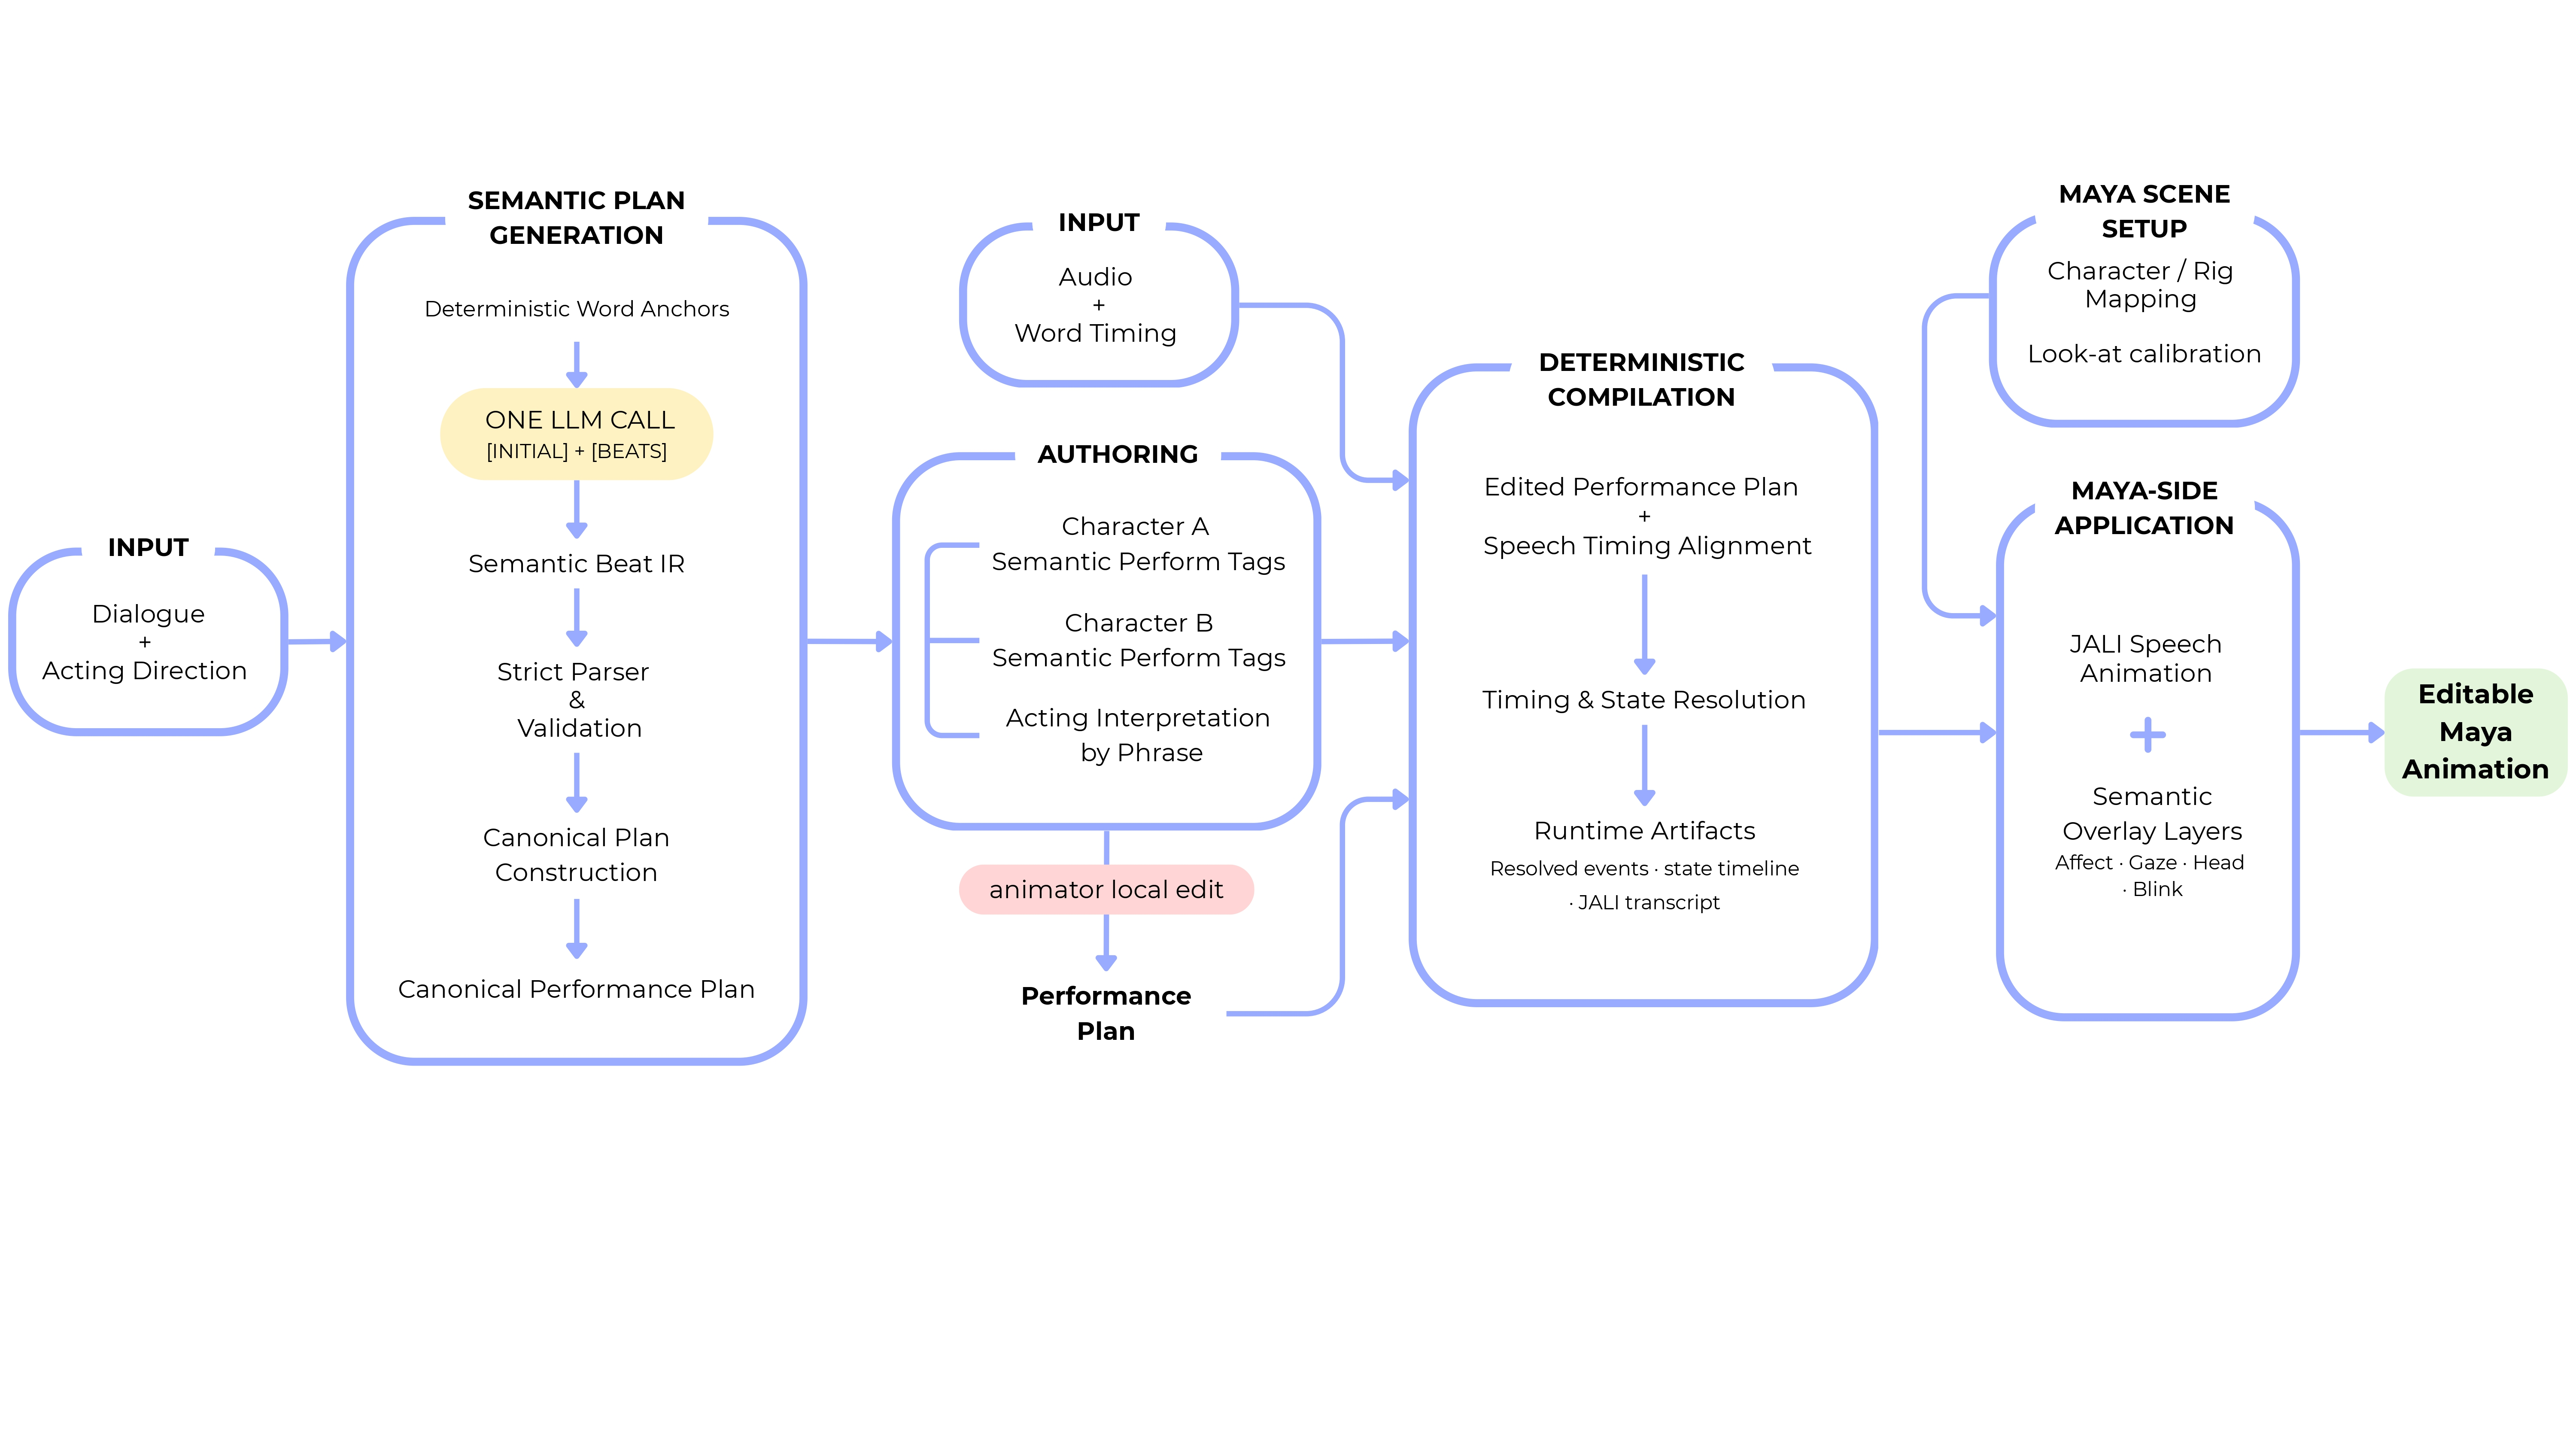
\includegraphics[width=\textwidth]{figures/system_architecture.jpg}
    \caption{System architecture. A single LLM call proposes a shared dyadic semantic interpretation over deterministic dialogue anchors. The canonical backend plan is exposed in Maya as character-specific Semantic Performance Tags; animator edits are resolved and compiled without another LLM call before deterministic JALI and Maya-side application.}
    \Description{A pipeline from dialogue and optional Acting Direction through deterministic word anchors, one LLM call, a validated canonical plan, Semantic Performance Tag authoring, deterministic timing and runtime compilation, and Maya-side speech, affect, gaze, head, and blink application.}
    \label{fig:system-overview}
\end{figure*}

\subsection{Anchored Conversational Context and Performance Interpretation}

The workflow begins with labeled dyadic dialogue, an optional free-text \textit{Acting Direction}, and two explicit character identities. Acting Direction may contain scene information, motivation, relationship context, or performance constraints; identities remain immutable throughout generation.

Before the model call, the system converts dialogue into ordered turns and global word anchors (\texttt{w0001}, \texttt{w0002}, \ldots), each retaining source text, speaker, turn, and position. The LLM selects semantic change points using these stable identifiers, which are reused for editing and timing resolution.

The prototype uses \texttt{gpt-5.6-luna} through the OpenAI API with medium reasoning effort and no task-specific training or fine-tuning. One model call receives immutable dialogue, anchored dialogue with speaker metadata, optional Acting Direction, the character-identity contract, and the executable semantic vocabulary. Output contains an initial state for both characters and sparse semantic beats. Initial states specify visible affect, persistent attention, optional head state, and a concise open-language acting interpretation. Each later beat belongs to one actor, is anchored to a dialogue word, and includes an acting interpretation plus at least one changed executable channel---affect, attention, head, or blink. Acting-only and redundant no-op beats are omitted.

The interpreter considers speaking and listening behavior independently. A listener reaction may be anchored to the earliest semantically sufficient word in the other character's speech rather than delayed to the turn boundary. Attention distinguishes persistent \texttt{focus: TARGET} from a temporary \texttt{eye\_action: brief\_check TARGET}; after validation these become author-facing \texttt{GAZE-*} and \texttt{GLANCE-*} tags, with glances returning to the prior persistent target. Targets may denote either interlocutor, another person, an object/location, or supported directional aversions. Executable affect, head, and blink values use finite supported vocabularies, while \texttt{acting} remains open language.

Model output is parsed and validated before authoring. Unsupported labels, unresolved identities, unknown anchors, malformed attention actions, and duplicate actor/anchor events are rejected rather than guessed. Valid beats compile into \texttt{dual\_performance\_plan\_v2}, which stores ordered identities, per-character initial states, sparse event tracks, semantic gaze-target candidates, and provenance. Redundant persistent no-op changes are removed deterministically while the original generated content remains in provenance.

\subsection{Semantic Performance Tag Authoring}

The Maya interface exposes the canonical plan as a readable projection rather than JSON (Figure~\ref{fig:interface}). In dual mode, each character has a separate Semantic Performance Tag panel over the same immutable dialogue. Dialogue spoken by that panel's character and dialogue heard from the interlocutor are visually distinguished, while tags are rendered separately, making both speaking and listening behavior visible within one conversational timeline. Unlike director-authored transcript tags such as those used by S$^3$ \cite{pan2024s3}, these tags are projected from the model-proposed plan and remain editable before execution.

\begin{figure*}[t]
    \centering
    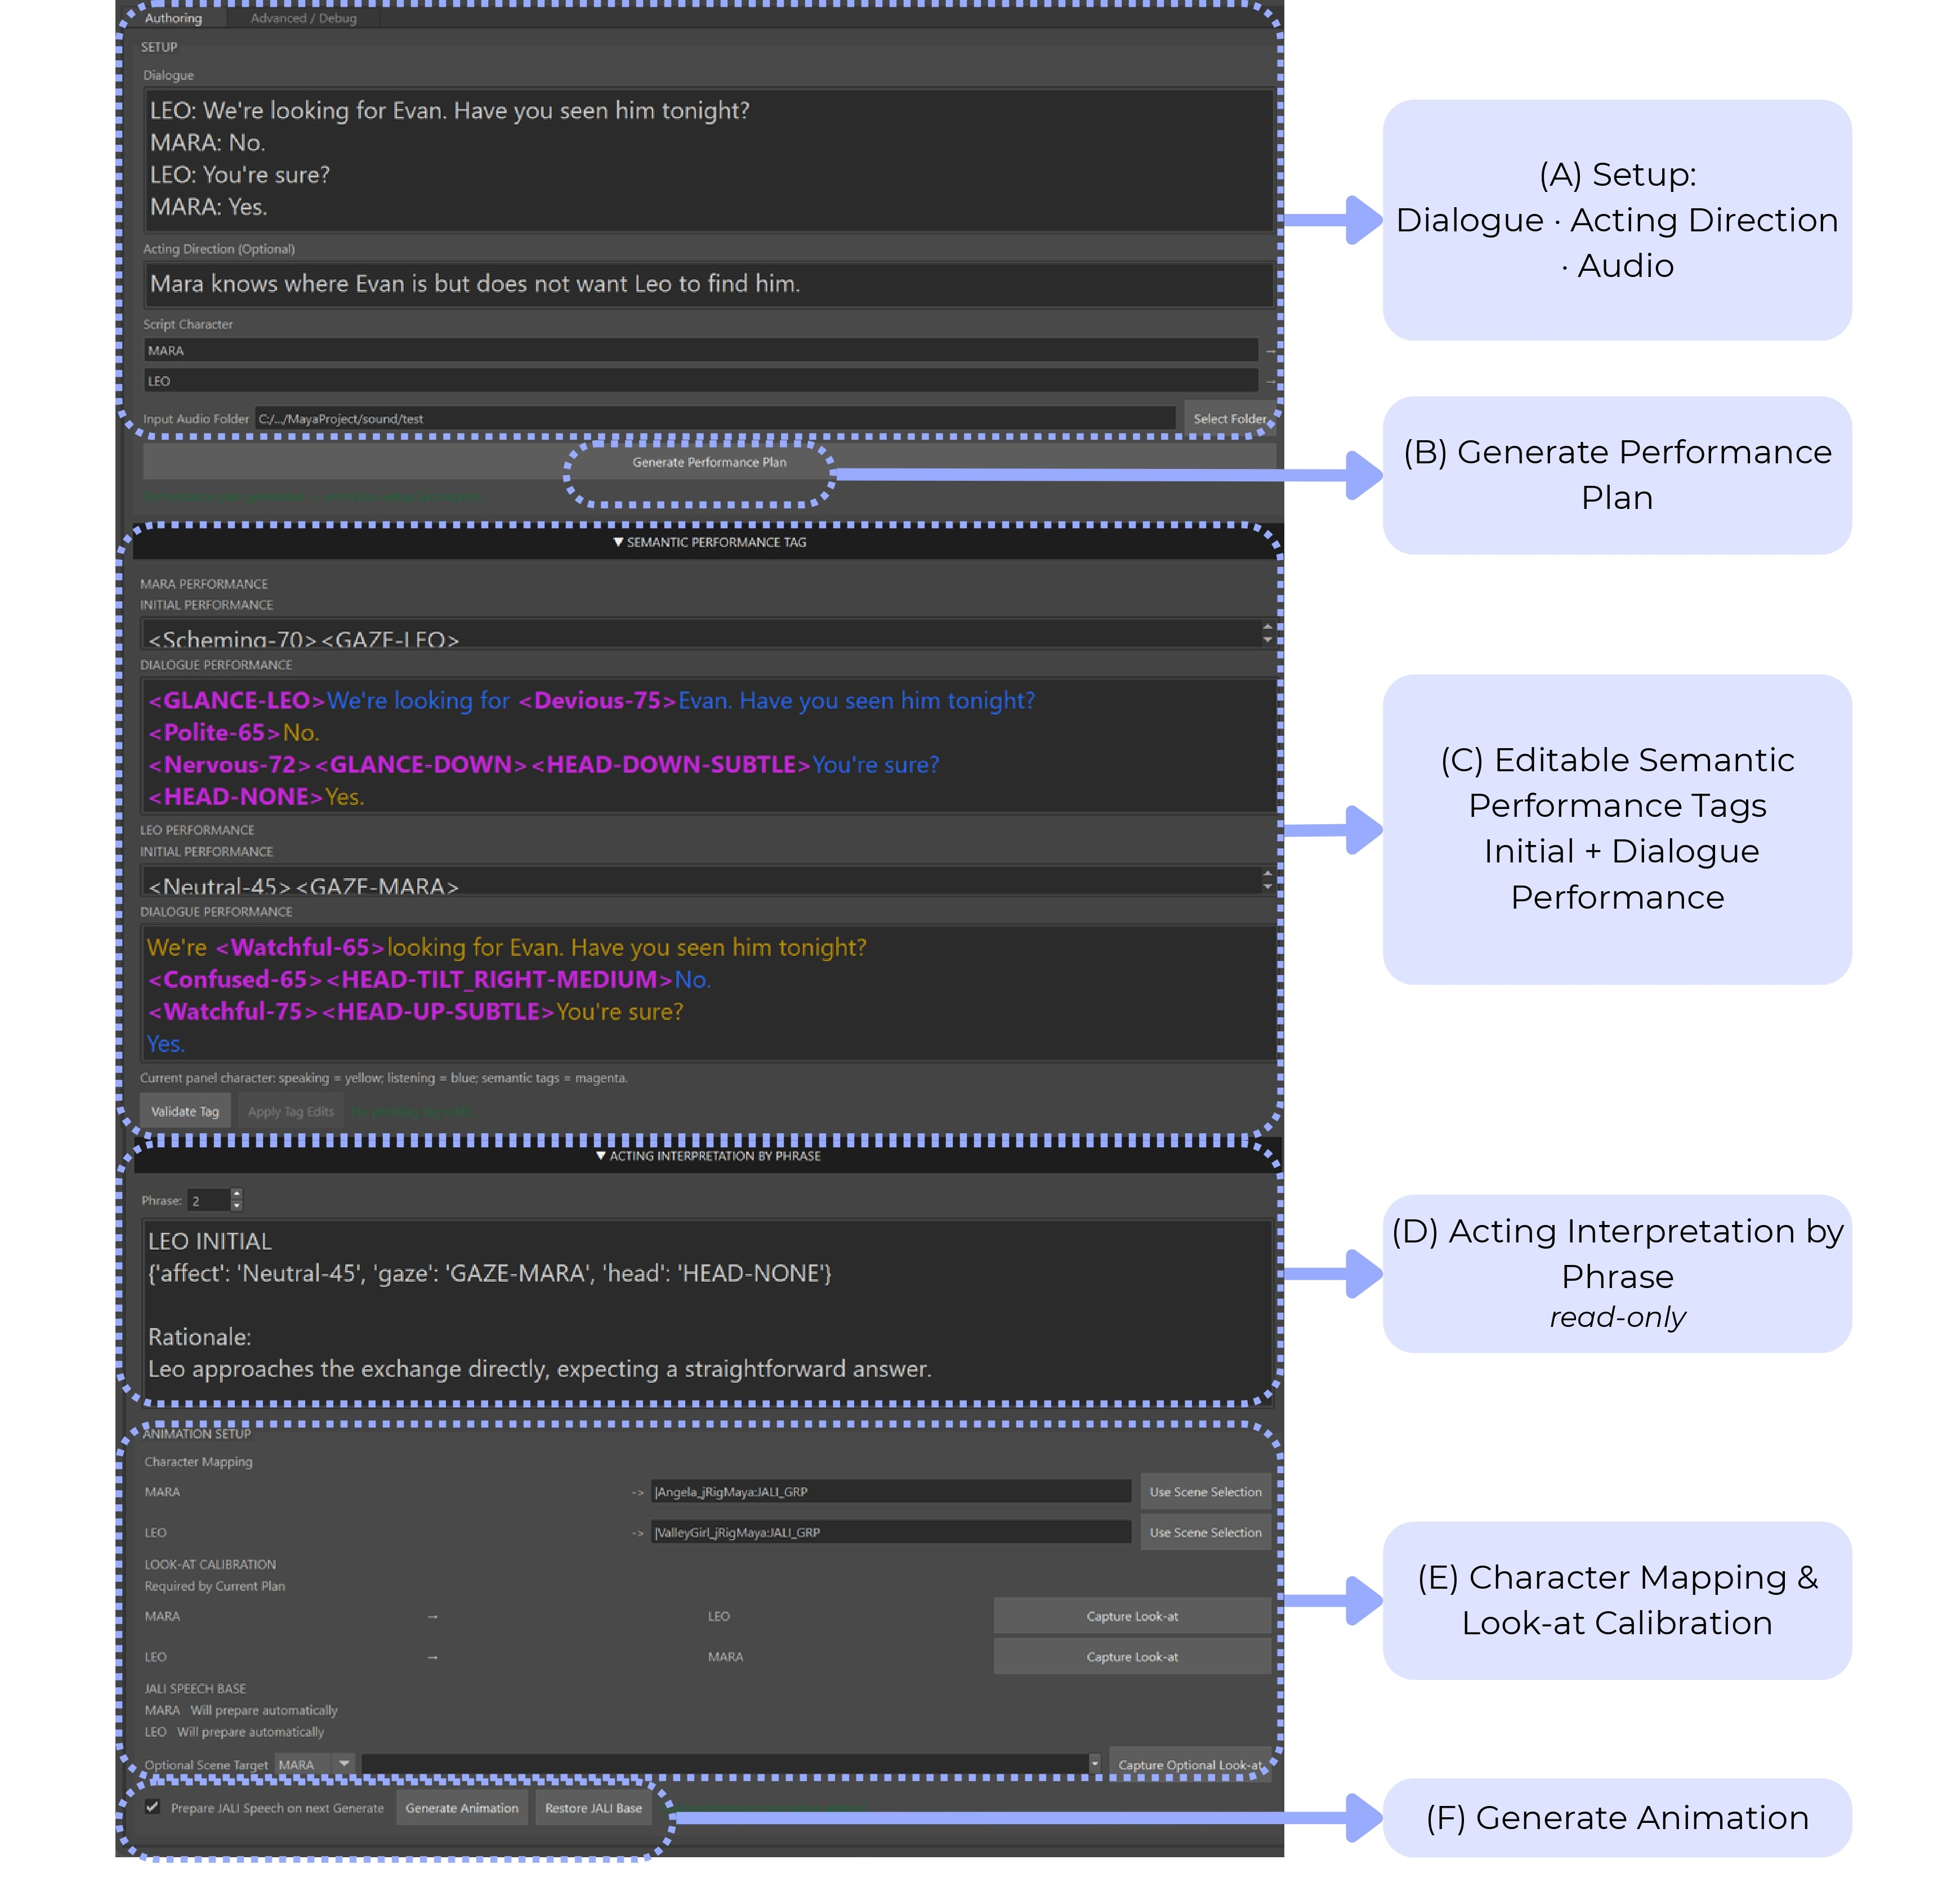
\includegraphics[width=\textwidth]{figures/ui_image.jpg}
    \caption{Participant-facing Maya interface with a filled dyadic example. The interface exposes dialogue and Acting Direction input, generation, editable Semantic Performance Tags for both characters, read-only \textit{Acting Interpretation by Phrase}, character mapping and look-at calibration, and animation generation.}
    \Description{An annotated Maya interface showing a filled dialogue and acting-direction example, the Generate Performance Plan control, two character-specific Semantic Performance Tag editors with initial and dialogue performance, the read-only Acting Interpretation by Phrase section, mapping and calibration, and Generate Animation.}
    \label{fig:interface}
\end{figure*}

Initial persistent state appears before dialogue; later changes appear as compact tags at their anchors. The current editable channels are visible affect, gaze/attention, head behavior, and performative blink. Users may change, add, remove, or reposition valid tag clusters across either character, including several semantic channels in one authoring pass. Dialogue tokens remain immutable, and validation checks the edited projection against the canonical dialogue and executable vocabulary.

Three interface operations separate generation from local editing. \textit{Generate Performance Plan} invokes the backend and loads a validated plan; \textit{Validate Tag} checks local edits without modifying the canonical plan; and \textit{Apply Tag Edits} writes valid edits into the in-memory plan without another LLM call. The original generated acting interpretation associated with each initial state or beat remains visible in a read-only \textit{Acting Interpretation by Phrase} view. When a generated tag is edited, its original interpretation is retained as provenance but marked stale; user-added changes have no original model interpretation.

Rig mappings, audio, and semantic-target-to-Maya look-at calibration remain outside the semantic representation. For each actor--target pair, the animator captures a visually appropriate gaze pose in the current shot. That pose becomes the execution target for a semantic directive such as \texttt{GAZE-B}. The semantic tag therefore does not encode a fixed world-space position or eye rotation. Thus one semantic attention decision can be retained while its visual realization is recalibrated for different cameras, staging, or rigs.

\subsection{Deterministic Compilation to JALI and Maya}

\textit{Generate Animation} treats the edited canonical plan as the source of truth. The LLM does not generate frames, rig coordinates, or animation curves. Instead, the compiler resolves semantic anchors against each character's word-level speech alignment (\texttt{words.jsonl} or a TextGrid \texttt{words} tier). A beat on a character's own word begins at that word's aligned start; a listener beat triggered by the other character begins at the end of the heard word. Persistent affect, gaze, and head state propagate forward, while glances and performative blinks remain event-local.

JALI supplies speech-driven facial animation and executable affect states \cite{edwards2016jali}. For each speaker, the backend constructs an annotated JALI transcript from the resolved affect state over aligned spoken words. Gaze, head, and blink remain in the resolved sparse event representation for deterministic Maya-side application. Persistent focus becomes \texttt{GAZE-*}; a temporary check becomes \texttt{GLANCE-*} and returns to the previously active persistent target. This tagged control abstraction is similar to S$^3$ \cite{pan2024s3}, but here directives are compiled from the edited semantic plan rather than supplied as director-authored transcript input. Character/object targets use calibrated Maya mappings, while directional targets use rig-relative offsets.

\begin{table}[t]
    \centering
    \caption{Mapping from author-facing Semantic Performance Tags to deterministic execution.}
    \label{tab:jiali-mapping}
    \begin{tabular}{p{0.27\columnwidth} p{0.63\columnwidth}}
        \toprule
        \textbf{Semantic field} & \textbf{Deterministic execution} \\
        \midrule
        Acting interpretation &
        Author-facing description; not mapped directly to a rig control. \\

        Affect / intensity &
        Resolved into supported JALI Mask states over aligned speech. \\

        Persistent \texttt{GAZE-*} &
        Maintains the semantic target until a later persistent gaze change. \\

        Temporary \texttt{GLANCE-*} &
        Produces a brief check and returns to the prior target. \\

        Head &
        Compiled to the supported head-control overlay vocabulary. \\

        Blink &
        Compiled to authored eyelid events such as slow/double blinks or eye-close/open holds. \\
        \bottomrule
    \end{tabular}
\end{table}

The compiler writes a dual animation manifest plus resolved per-character events, persistent state timelines, and JALI-annotated transcripts. Maya-side applicators use these artifacts, calibrated look-at poses, and mapped rigs to construct affect, gaze, head, and blink layers. The design boundary is therefore explicit: the LLM proposes \textit{what} the performance means and where semantic changes occur; deterministic code decides \textit{how} those decisions are validated, aligned, and instantiated as animation.
